% \documentclass[aspectratio=169, 11pt]{beamer}
\documentclass[aspectratio=169, 11pt, handout]{beamer}

% Version 2 (2026-09-28). Restructured on the course spine: estimand -> identification -> estimation
% (course-spine.md). Changes from slides.tex are listed in m01/CHANGES-v2.md.

% ── Theme ──
\usetheme{Madrid}
\usecolortheme{default}
\setbeamertemplate{navigation symbols}{}
\setbeamertemplate{footline}{%
  \leavevmode\hbox{%
    \begin{beamercolorbox}[wd=.333333\paperwidth,ht=2.5ex,dp=1ex,center]{author in head/foot}%
      \usebeamerfont{author in head/foot}\insertshortauthor
    \end{beamercolorbox}%
    \begin{beamercolorbox}[wd=.333333\paperwidth,ht=2.5ex,dp=1ex,center]{title in head/foot}%
      \usebeamerfont{title in head/foot}\insertshorttitle
    \end{beamercolorbox}%
    \begin{beamercolorbox}[wd=.333333\paperwidth,ht=2.5ex,dp=1ex,right]{date in head/foot}%
      \usebeamerfont{date in head/foot}\insertframenumber{} / \inserttotalframenumber\hspace*{2ex}
    \end{beamercolorbox}}}

% ── Packages ──
\usepackage{amsmath,amssymb}
\usepackage{booktabs}
\usepackage{xcolor}
\usepackage{colortbl}
\usepackage{graphicx}
\usepackage{tikz}
\usetikzlibrary{arrows.meta, positioning, calc}

% ── Colors ──
\definecolor{sbgreen}{HTML}{00704A}  % course accent
\definecolor{warnred}{HTML}{CC0000}
\definecolor{noteblue}{HTML}{2060A0}

% ── Commands ──
\newcommand{\E}{\mathbb{E}}
\newcommand{\Var}{\mathrm{Var}}
\newcommand{\Cov}{\mathrm{Cov}}
\newcommand{\SE}{\mathrm{SE}}
\newcommand{\Prob}{\mathrm{Pr}}
\newcommand{\indep}{\perp\!\!\!\perp}
\usepackage{soul}
\newcommand{\NUM}[2]{\sethlcolor{yellow}\hl{#1\,\textsuperscript{?}}\marginpar{\tiny #2}}
% Beamer frames are typeset inside boxes, where \marginpar raises "Not in outer par mode"
% and \marginparwidth is 4pt. Same marker; the provenance note goes to the frame footnote.
\renewcommand{\NUM}[2]{\sethlcolor{yellow}\hl{#1\,\textsuperscript{?}}\footnote[frame]{\tiny #2}}
% Compact footnote layout so several provenance notes fit under one frame.
\setbeamertemplate{footnote}{\noindent\raggedright\hspace*{0.6em}\tiny\insertfootnotemark\,\insertfootnotetext\par}

% Step labels for the course spine
\newcommand{\spinestep}[1]{\textcolor{sbgreen}{\textbf{#1}}}

% ── Title ──
\title[Meeting 1]{Meeting 1: The Coupon and the Coin}
\subtitle{Applied Causal Inference for Business}
\author{Zhikun Lu}
\date{\today}

\begin{document}

% ====================================================================
\begin{frame}
\titlepage
\end{frame}

% ====================================================================
\begin{frame}{Where Does the Counterfactual Come From?}

\begin{center}
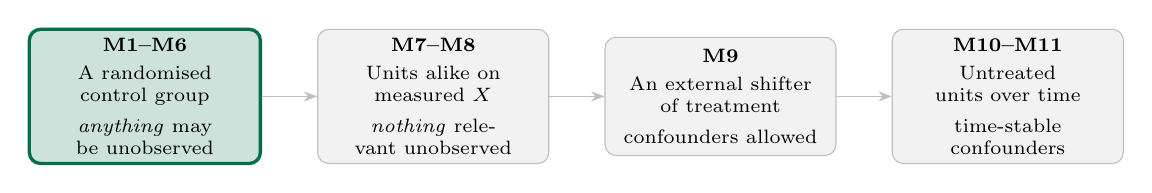
\begin{tikzpicture}[
    node distance=0.45cm and 0.7cm,
    box/.style={draw, rounded corners, minimum width=2.9cm, minimum height=1.5cm,
                font=\scriptsize, align=center, text width=2.7cm},
    active/.style={box, fill=sbgreen!20, draw=sbgreen, very thick},
    inactive/.style={box, fill=gray!10, draw=gray!50}
]
\node[active] (A) {\textbf{M1--M6}\\[2pt] A randomised control group\\[3pt] \emph{anything} may be unobserved};
\node[inactive, right=of A] (B) {\textbf{M7--M8}\\[2pt] Units alike on measured $X$\\[3pt] \emph{nothing} relevant unobserved};
\node[inactive, right=of B] (C) {\textbf{M9}\\[2pt] An external shifter of treatment\\[3pt] confounders allowed};
\node[inactive, right=of C] (D) {\textbf{M10--M11}\\[2pt] Untreated units over time\\[3pt] time-stable confounders};

\draw[-{Stealth}, gray!50] (A) -- (B);
\draw[-{Stealth}, gray!50] (B) -- (C);
\draw[-{Stealth}, gray!50] (C) -- (D);
\end{tikzpicture}
\end{center}

\bigskip

\begin{center}
\small Every decision in this course needs the same missing number: what \emph{would} have happened.\\
Four answers to where it comes from. Today, the first: a coin decides who is treated.
\end{center}
\end{frame}

% ====================================================================
\begin{frame}{Three Steps, Every Meeting}

\begin{center}
\begin{tabular}{p{3.0cm}p{9.6cm}}
\toprule
\spinestep{1. Estimand} & The causal number the decision needs --- for which units, which intervention against which alternative, which outcome, over what horizon. Written in potential outcomes \emph{before} any data. \\[0.5em]
\spinestep{2. Identification} & How treatment was assigned, and what must be true for the data to reveal the estimand. Every assumption tied to a fact about the procedure. \\[0.5em]
\spinestep{3. Estimation} & A formula to compute it from the data, and its uncertainty --- which comes from the design: what was random, and at what level. \\
\bottomrule
\end{tabular}
\end{center}

\bigskip

Methods --- regression, machine learning, instruments, panels --- live in step~3. They compute an identified quantity. \textbf{They never identify it.}

\medskip

\small AI makes step~3 cheap. Steps 1 and 2 are the scarce skill.
\end{frame}

% ====================================================================
\begin{frame}{Today's Plan}

\begin{enumerate}
    \item \spinestep{Estimand:} a coupon rollout, the number that settles it, and two worlds for every customer
    \item \spinestep{Identification:} why the pilot's comparison misleads --- and why a coin does not
    \item \spinestep{Estimation:} the difference in means, what ``unbiased'' means for one draw, and the regression that computes it
    \item What counts as a treatment
    \item What the coupon is worth, and to whom
\end{enumerate}

\bigskip

\textbf{Case:} Lin's coupon programme, Meeting 1 (Releases 1--5). \quad \textbf{Workshop, no AI:} arm means, label reversal, seeds.

\bigskip

\textbf{Reading:} technical notes for Meeting 1. Section 1 is examinable; Section 3 and \emph{Extensions} are reference.
\end{frame}

% ====================================================================
\section{The Estimand}
% ====================================================================

% [RELEASE R1 — narrative and marketing's pilot numbers]
\begin{frame}{The Coffee Chain, Before the Experiment}

\textbf{Lin} runs customer analytics for a coffee chain with \textbf{10{,}000} loyalty members.

\bigskip

Marketing wants to send every member a coupon: \textyen 10 off the next purchase.

\bigskip
\pause

\textbf{Their evidence:} a Q1 pilot in one region of 1{,}000 members. The coupon went to 500 of them --- the ones marketing judged most loyal.

\begin{center}
\small
\begin{tabular}{lrr}
\toprule
& \textbf{Got coupon} & \textbf{No coupon} \\
\midrule
Purchase rate & 0.68 & 0.24 \\
\bottomrule
\end{tabular}
\end{center}

\smallskip
\begin{center}
Marketing's reading: \emph{``The coupon lifts purchases by 44 points. Send it to everyone.''}
\end{center}
\end{frame}

% ====================================================================
\begin{frame}{The Number That Decides It}

A purchase earns \textyen 30 of margin. The coupon costs \textyen 10, paid on \emph{every} purchase a coupon holder makes --- including the ones they would have made anyway.

\bigskip

Per coupon sent, with $p_1$ the purchase rate among holders and $\tau$ the lift the coupon causes:
\[
\text{net} \;=\; \underbrace{\tau \times 30}_{\text{purchases the coupon caused}} \;-\; \underbrace{10 \times p_1}_{\text{coupons redeemed}} .
\]

\pause

\begin{alertblock}{Break-even lift}
\[
\tau^{*} \;=\; \frac{10\, p_1}{30} \;=\; \frac{p_1}{3}
\]
\end{alertblock}

\medskip

Marketing's numbers: $p_1 = 0.68$, so $\tau^* = 0.227$. Their lift of $0.44$ gives $0.44 \times 30 - 6.8 = +$\textyen 6.40 per coupon, \textbf{+\textyen 64{,}000} across the base.

\medskip

Every estimate today is a lift. The only question is \textbf{which side of $p_1/3$} it lands on.
\end{frame}

% [CARRIED VERBATIM from old-decks/lecture01.tex:121]
\begin{frame}{The Prediction Approach (and Why It Fails)}

\textbf{Natural idea:} Build a model to predict who will buy, then send coupons to high-probability customers.

\bigskip

\textbf{Problem:} The model predicts $\Prob(\text{purchase} \mid X)$, not the \emph{causal effect} of the coupon.

\bigskip

\begin{center}
\begin{tabular}{lcc}
\toprule
\textbf{Customer} & \textbf{P(buy)} & \textbf{Effect of coupon} \\
\midrule
Daily regular & 0.95 & $\approx 0$ (buys anyway) \\
Lapsed customer & 0.05 & could be large \\
\bottomrule
\end{tabular}
\end{center}

\bigskip

Prediction targets the \emph{wrong column}. We need the \emph{missing column}: the causal effect.
\end{frame}

% ====================================================================
\begin{frame}{The Four Types of Customers}

For each customer, imagine \textbf{two worlds}: one with coupon, one without.

\bigskip

\begin{center}
\begin{tabular}{l|c|c|}
\multicolumn{1}{c}{} & \multicolumn{1}{c}{\textbf{Doesn't buy with coupon}} & \multicolumn{1}{c}{\textbf{Buys with coupon}} \\
\cline{2-3}
\textbf{Doesn't buy without} & \cellcolor{gray!15} Lost Cause & \cellcolor{green!15} \textbf{Persuadable} \\
& ITE $= 0$ & ITE $= +1$ \\
\cline{2-3}
\textbf{Buys without} & \cellcolor{red!15} Do-Not-Disturb & \cellcolor{blue!10} Sure Thing \\
& ITE $= -1$ & ITE $= 0$ \\
\cline{2-3}
\end{tabular}
\end{center}

\bigskip

\begin{itemize}
    \item \textbf{Persuadable:} coupon \emph{causes} a purchase
    \item \textbf{Sure Thing:} buys anyway --- the coupon discounts a purchase that was coming
    \item \textbf{Lost Cause:} never buys --- the coupon goes unused
    \item \textbf{Do-Not-Disturb:} coupon \emph{prevents} a purchase
\end{itemize}

\small Types are a thought device: nobody's type is ever observed.
\end{frame}

% ====================================================================
\begin{frame}{What Each Type Costs}

Change in margin from sending one coupon. \textyen 30 per purchase; the \textyen 10 is paid only when the coupon is used; no contact fee today.

\bigskip

\begin{center}
\begin{tabular}{lrrr}
\toprule
\textbf{Type} & \textbf{Without coupon} & \textbf{With coupon} & \textbf{Change} \\
\midrule
Persuadable & 0 & 20 & \textcolor{sbgreen}{$+20$} \\
Sure Thing & 30 & 20 & \textcolor{warnred}{$-10$} \\
Lost Cause & 0 & 0 & $0$ \\
Do-Not-Disturb & 30 & 0 & \textcolor{warnred}{$-30$} \\
\bottomrule
\end{tabular}
\end{center}

\bigskip

Average over any mix of types:
\[
\text{net} = 20\,p_1 - 30\,p_0 = 30\tau - 10\,p_1 .
\]

\textbf{The expensive customer is the Sure Thing, not the Lost Cause.} A coupon nobody uses costs nothing here; in M6 a contact fee changes that.
\end{frame}

% [CARRIED VERBATIM from old-decks/lecture01.tex:180]
\begin{frame}{The Fundamental Problem}

\begin{alertblock}{Key Insight}
For each customer, we observe \textbf{only one} of the two worlds.
\end{alertblock}

\bigskip

\begin{itemize}
    \item If customer $i$ gets the coupon, we see whether they buy \emph{with} the coupon
    \item We \textbf{never} see what they would have done \emph{without} it
    \item The other outcome is the \textbf{counterfactual}
\end{itemize}

\bigskip

This means:
\begin{itemize}
    \item We cannot classify any individual into one of the four types
    \item We need a strategy that works at the \emph{population} level
\end{itemize}
\end{frame}

% [CARRIED VERBATIM from old-decks/lecture01.tex:208, SUTVA line added]
\begin{frame}{Formalizing Counterfactuals}

\textbf{Notation.} For each individual $i$:

\medskip

\begin{center}
\begin{tabular}{ll}
$D_i \in \{0, 1\}$ & treatment assignment (1 = coupon, 0 = no coupon) \\[0.3em]
$Y_i(1)$ & \textbf{potential outcome} if treated \\[0.3em]
$Y_i(0)$ & \textbf{potential outcome} if not treated \\[0.3em]
$\tau_i = Y_i(1) - Y_i(0)$ & \textbf{individual treatment effect} (ITE)
\end{tabular}
\end{center}

\bigskip

\textbf{Observed outcome} (consistency):
\[
Y_i = D_i \cdot Y_i(1) + (1 - D_i) \cdot Y_i(0)
\]

\medskip

We see $Y_i(1)$ if treated, $Y_i(0)$ if not. Never both.

\medskip

\small Writing $Y_i(d)$ with one index assumes one version of the coupon and that my outcome does not depend on your coupon (SUTVA). M2 checks both.
\end{frame}

% ====================================================================
\begin{frame}{The Estimand: Say It in a Sentence First}

\emph{``The average effect of sending this \textyen 10 app coupon, against sending nothing, on a purchase within seven days, among \underline{these} customers.''}

\bigskip

\begin{center}
\begin{tabular}{lll}
\toprule
\textbf{Estimand} & \textbf{Definition} & \textbf{Averages over} \\
\midrule
ATE & $\tau = \E[Y(1) - Y(0)]$ & everyone in the population \\
ATT & $\E[Y(1) - Y(0) \mid D = 1]$ & those who got the coupon \\
ATU & $\E[Y(1) - Y(0) \mid D = 0]$ & those who did not \\
\bottomrule
\end{tabular}
\end{center}

\bigskip

Linked by $\tau = \Prob(D = 1)\,\tau_{\text{ATT}} + \Prob(D = 0)\,\tau_{\text{ATU}}$. In response types, $\tau = \Prob(\text{Persuadable}) - \Prob(\text{Do-Not-Disturb})$.

\bigskip

\textbf{Which population?} The 1{,}000 members of the test region are where an effect can be \emph{measured}; the 10{,}000-member base is where the decision \emph{lands}. Today's estimand is the first. Moving it to the second is a separate step (M2).
\end{frame}

% ====================================================================
\section{Identification: Why the Pilot Misleads}
% ====================================================================

% [CARRIED VERBATIM from old-decks/lecture01.tex:279]
\begin{frame}{The Naive Comparison and Why It Fails}

\textbf{Natural idea:} Compare outcomes between treated and untreated groups.
\[
\text{``Effect''} = \E[Y \mid D = 1] - \E[Y \mid D = 0]
\]

\textbf{Problem:} This equals the ATE \emph{only if} the groups are comparable.

\bigskip

If the marketing team targets coupons at loyal customers:
\begin{itemize}
    \item Coupon group: packed with \textbf{Sure Things} (buy anyway)
    \item No-coupon group: more \textbf{Lost Causes} (don't buy anyway)
    \item The coupon \emph{looks} effective, but the groups were different to begin with
\end{itemize}

\bigskip

This is \textbf{confounding}: the way treatment was \emph{assigned} (by loyalty) is related to the outcome.
\end{frame}

% [RELEASE R2 — the warm-up records, then the pilot region's type counts (a thought experiment: nobody observes types)]
\begin{frame}{Board Task: What Can We Fill In?}

Four customers from the pilot. Fill in only what was observed.

\bigskip

\begin{center}
\begin{tabular}{crrccl}
\toprule
\textbf{Customer} & $D$ & $Y$ & $Y(1)$ & $Y(0)$ & \textbf{Compatible types} \\
\midrule
A & 1 & 1 & 1 & ? & Sure Thing or Persuadable \\
B & 0 & 1 & ? & 1 & Sure Thing or Do-Not-Disturb \\
C & 1 & 0 & 0 & ? & Lost Cause or Do-Not-Disturb \\
D & 0 & 0 & ? & 0 & Lost Cause or Persuadable \\
\bottomrule
\end{tabular}
\end{center}

\bigskip

\small (Handout: attempt before this frame; the last three columns are the answer.)

\normalsize
\bigskip

More customers help us estimate \textbf{averages}. They never reveal A's missing outcome.
\end{frame}

% [CARRIED VERBATIM from old-decks/lecture01.tex:309]
\begin{frame}{Confounding: A Numerical Example}

True type distribution: 1,000 customers.

\bigskip

\begin{center}
\begin{tabular}{lrc}
\toprule
\textbf{Type} & \textbf{Count} & \textbf{Share} \\
\midrule
Lost Cause (0,0) & 400 & 40\% \\
Sure Thing (1,1) & 300 & 30\% \\
Persuadable (0,1) & 200 & 20\% \\
Do-Not-Disturb (1,0) & 100 & 10\% \\
\bottomrule
\end{tabular}
\end{center}

\bigskip

True ATE $= 0.50 - 0.40 = \mathbf{0.10}$ (10 pp).
\end{frame}

% Worksheet: pairs compute both arms' purchase rates from the counts before the \pause reveal.
% [CARRIED VERBATIM from old-decks/lecture01.tex:331]
\begin{frame}{Confounded Assignment}

Marketing targets 500 loyal customers $\Rightarrow$ Sure Things overrepresented in coupon group:

\bigskip

\begin{center}
\begin{tabular}{lccr}
\toprule
\textbf{Type} & \textbf{Coupon (500)} & \textbf{No-coupon (500)} & \textbf{Total} \\
\midrule
Lost Cause (0,0) & 100 & 300 & 400 \\
Sure Thing (1,1) & \textcolor{warnred}{220} & 80 & 300 \\
Persuadable (0,1) & 120 & 80 & 200 \\
Do-Not-Disturb (1,0) & 60 & 40 & 100 \\
\bottomrule
\end{tabular}
\end{center}

\pause

\begin{align*}
\text{Purchase rate (coupon)} &= (220 + 120)/500 = 0.68 \\
\text{Purchase rate (no-coupon)} &= (80 + 40)/500 = 0.24 \\
\text{Naive difference} &= 0.68 - 0.24 = \textcolor{warnred}{0.44}
\end{align*}

\textbf{4.4$\times$ the true effect!} Sure Things inflate the coupon group's success rate.
\end{frame}

% [CARRIED VERBATIM from old-decks/lecture02.tex:248]
\begin{frame}{Selection Bias Decomposition}

Can we estimate the ATE from observed data?
\[
\E[Y \mid D\!=\!1] - \E[Y \mid D\!=\!0] \stackrel{?}{=} \tau
\]

\begin{block}{Proposition: Selection Bias Decomposition}
\[
\underbrace{\E[Y \mid D\!=\!1] - \E[Y \mid D\!=\!0]}_{\text{Naive comparison}} = \underbrace{\E[Y(1)\!-\!Y(0) \mid D\!=\!1]}_{\text{ATT}} + \underbrace{\E[Y(0) \mid D\!=\!1] - \E[Y(0) \mid D\!=\!0]}_{\textcolor{warnred}{\text{Selection Bias}}}
\]
\end{block}

\medskip

\textbf{Proof:} consistency, then add and subtract $\E[Y(0) \mid D = 1]$ --- the one number the data never show.

\bigskip

\textbf{Selection bias} $\neq 0$ whenever the treated and untreated would have had different outcomes \emph{even without treatment}.
\end{frame}

% ====================================================================
\begin{frame}{The Pilot, Decomposed}

Read the decomposition off the pilot's type counts. $Y(0) = 1$ for Sure Things and Do-Not-Disturbs.

\begin{center}
\small
\begin{tabular}{lrr}
\toprule
& \textbf{Coupon (500)} & \textbf{No coupon (500)} \\
\midrule
Would buy \emph{without} the coupon: ST $+$ DND & $220 + 60 = 280$ & $80 + 40 = 120$ \\
$\E[Y(0) \mid D]$ & $0.56$ & $0.24$ \\
\bottomrule
\end{tabular}
\end{center}

\begin{align*}
\text{ATT} &= \frac{\#\text{Persuadable} - \#\text{DND}}{500} = \frac{120 - 60}{500} = 0.12 \\
\text{selection bias} &= 0.56 - 0.24 = 0.32 \\
\text{naive} &= 0.12 + 0.32 = \textcolor{warnred}{0.44}
\end{align*}

Three quarters of marketing's lift is \textbf{who they picked}, not what the coupon did. Even for the pilot's own recipients, $0.12 < 0.227$:
\[
0.12 \times 30 - 6.8 = \textcolor{warnred}{-\text{\textyen}3.20 \text{ per coupon}}.
\]
\end{frame}

% ====================================================================
\begin{frame}{Two Kinds of Selection}

The non-recipients' effect, from the same table:
\[
\tau_{\text{ATU}} = \frac{80 - 40}{500} = 0.08, \qquad \tfrac12(0.12) + \tfrac12(0.08) = 0.10 = \tau \;\checkmark
\]

\bigskip

Against the ATE, the pilot's 0.44 is off by $0.34$, for two separate reasons:

\medskip

\begin{center}
\small
\begin{tabular}{lrl}
\toprule
\textbf{Source} & \textbf{Size} & \textbf{What marketing did} \\
\midrule
Baseline selection: $\E[Y(0) \mid D=1] - \E[Y(0) \mid D=0]$ & $0.32$ & picked people who buy anyway \\
Selection on gains: $\tau_{\text{ATT}} - \tau$ & $0.02$ & picked slightly better responders \\
\bottomrule
\end{tabular}
\end{center}

\bigskip

A larger pilot would estimate $0.44$ more precisely. \textbf{It would not move it toward $0.10$.} Bias is about the assignment, not the sample size.
\end{frame}

% ====================================================================
\begin{frame}{Two Kinds of Customer}

Lin's CRM splits the whole base into two segments of 5{,}000. Take the segment effects as given for now --- estimating them is M3.

\bigskip

\begin{center}
\begin{tabular}{lccc}
\toprule
\textbf{Segment} & $\E[Y(1) \mid X]$ & $\E[Y(0) \mid X]$ & \textbf{Effect} \\
\midrule
Active ($X = 1$) & 0.80 & 0.75 & $+0.05$ \\
Lapsed ($X = 0$) & 0.30 & 0.10 & $+0.20$ \\
\bottomrule
\end{tabular}
\end{center}

\[
\tau = 0.5 \times 0.05 + 0.5 \times 0.20 = \mathbf{0.125}
\]

The coupon works four times better on customers who were drifting away. Active customers buy anyway.

\bigskip

\small This is a different population from the pilot region, and it has a different ATE. Both are real answers; neither is \emph{the} effect. That is why step 1 names the population.
\end{frame}

% [RELEASE R3 — two targeting policies; pairs compute both before the reveal]
\begin{frame}{Who Got the Coupon Decides the Sign}

Two ways a manager might have run the pilot on the whole base. Treated $=$ one segment, control $=$ the other.

\begin{columns}[T]
\begin{column}{0.49\textwidth}
\textbf{Coupon to the active}
\begin{align*}
\E[Y \mid D = 1] &= 0.80 \\
\E[Y \mid D = 0] &= 0.10 \\
\text{naive} &= \textcolor{warnred}{+0.70}
\end{align*}
\[
\underbrace{0.70}_{\text{naive}} = \underbrace{0.05}_{\text{ATT}} + \underbrace{0.75 - 0.10}_{\text{bias} \,=\, +0.65}
\]
\small Active customers buy anyway: a 14-fold \textbf{overestimate}.
\end{column}
\begin{column}{0.49\textwidth}
\textbf{Coupon to the lapsed}
\begin{align*}
\E[Y \mid D = 1] &= 0.30 \\
\E[Y \mid D = 0] &= 0.75 \\
\text{naive} &= \textcolor{warnred}{-0.45}
\end{align*}
\[
\underbrace{-0.45}_{\text{naive}} = \underbrace{0.20}_{\text{ATT}} + \underbrace{0.10 - 0.75}_{\text{bias} \,=\, -0.65}
\]
\small The coupon looks harmful. It lifts the lapsed by 20 points: a \textbf{sign reversal}.
\end{column}
\end{columns}

\bigskip

\begin{center}
Same coupon, same customers. The sign is set by \textbf{who was chosen}. Keep the right-hand column: it comes back in M7.
\end{center}
\end{frame}

% ====================================================================
\section{Identification by Design: The Coin}
% ====================================================================

% [RELEASE R4 — the Q2 randomised test in the pilot region]
% [CARRIED VERBATIM from old-decks/lecture01.tex:364]
\begin{frame}{The Solution: Randomization}

Randomly assign 500 customers to coupon, 500 to control.

\bigskip

\begin{center}
\begin{tabular}{lccr}
\toprule
\textbf{Type} & \textbf{Coupon (500)} & \textbf{No-coupon (500)} & \textbf{Total} \\
\midrule
Lost Cause (0,0) & 200 & 200 & 400 \\
Sure Thing (1,1) & \textcolor{sbgreen}{150} & \textcolor{sbgreen}{150} & 300 \\
Persuadable (0,1) & 100 & 100 & 200 \\
Do-Not-Disturb (1,0) & 50 & 50 & 100 \\
\bottomrule
\end{tabular}
\end{center}

\pause

\begin{align*}
\text{Purchase rate (coupon)} &= (150 + 100)/500 = 0.50 \\
\text{Purchase rate (no-coupon)} &= (150 + 50)/500 = 0.40 \\
\text{Difference} &= 0.50 - 0.40 = \textcolor{sbgreen}{\mathbf{0.10}} = \text{true ATE} \; \checkmark
\end{align*}

\small This table shows the \emph{expected} split. The next slide shows a draw that actually happens.
\end{frame}

% ====================================================================
\begin{frame}{A Random Draw Need Not Balance}

The same 1{,}000 customers; another draw the seed could have produced.

\bigskip

\begin{center}
\begin{tabular}{lrr}
\toprule
\textbf{Type} & \textbf{Coupon (500)} & \textbf{No coupon (500)} \\
\midrule
Lost Cause & 195 & 205 \\
Sure Thing & 155 & 145 \\
Persuadable & 105 & 95 \\
Do-Not-Disturb & 45 & 55 \\
\bottomrule
\end{tabular}
\end{center}

\[
\widehat\tau = \frac{155 + 105}{500} - \frac{145 + 55}{500} = 0.52 - 0.40 = \mathbf{0.12} \qquad \text{(true: } 0.10\text{)}
\]

\textbf{Nothing is broken.} Randomisation removes \emph{systematic} selection --- over all the draws the seed could make --- not the luck of this one. How far a single draw can land is this afternoon's workshop, and M2's first question.
\end{frame}

% [MERGED from old-decks/lecture01.tex:392 and lecture02.tex:364]
\begin{frame}{Identification Under Random Assignment}

\begin{block}{Assignment mechanism}
\[
D \indep \bigl(Y(0),\, Y(1)\bigr), \qquad 0 < \Prob(D = 1) < 1
\]
\end{block}

\begin{block}{Result: the ATE is identified}
Under consistency and random assignment,
\[
\tau = \E[Y(1)] - \E[Y(0)] = \E[Y \mid D = 1] - \E[Y \mid D = 0]
\]
\end{block}

\textbf{Proof:} consistency gives $\E[Y \mid D\!=\!1] = \E[Y(1) \mid D\!=\!1]$; independence gives $\E[Y(1) \mid D\!=\!1] = \E[Y(1)]$. Same for $D = 0$. Selection bias $= 0$, and $\tau = \tau_{\text{ATT}} = \tau_{\text{ATU}}$. $\square$

\bigskip

Independence is a property of the \textbf{procedure}, not the customers: a random number generator knows nothing about anyone's potential outcomes --- observed or not.
\end{frame}

% ====================================================================
\begin{frame}{Verifying with the Two Segments}

Under a random 50/50 split of the base, each arm is half active, half lapsed:

\begin{align*}
\E[Y \mid D = 1] &= 0.5 \times 0.80 + 0.5 \times 0.30 = 0.55 \\
\E[Y \mid D = 0] &= 0.5 \times 0.75 + 0.5 \times 0.10 = 0.425 \\
\text{Difference} &= 0.55 - 0.425 = \textcolor{sbgreen}{\mathbf{0.125}} = \tau \quad \checkmark
\end{align*}

\begin{block}{Under randomisation, all three averages coincide}
\[
\tau = \tau_{\text{ATT}} = \tau_{\text{ATU}} = 0.125
\]
\end{block}

Both arms are the population in miniature, so ``the treated'' and ``everyone'' are the same people in distribution. Compare the targeted pilots: ATT of $0.05$ or $0.20$, depending on who was picked.
\end{frame}

% ====================================================================
\begin{frame}{What Must Be True}

From Lin's description of the Q2 test:

\bigskip

\begin{center}
\small
\begin{tabular}{p{6.4cm}p{6.6cm}}
\toprule
\textbf{The case says} & \textbf{Which buys} \\
\midrule
``The 500 recipients were drawn by a random number generator; the seed is in the log.'' & Independence: $D \indep \{Y(0), Y(1)\}$. Nobody chose. \\[0.5em]
``Nobody could opt in, and nobody was removed after the draw.'' & Independence survives: the arms are still the draw. \\[0.5em]
``One coupon design, sent in the app, single-use and tied to the account.'' & Consistency: one version of treatment; codes cannot be passed on. \\[0.5em]
``Store staff did not know who held a coupon.'' & No other treatment travels with the coupon. \\
\bottomrule
\end{tabular}
\end{center}

\bigskip

\textbf{Every row can be checked from the logs.} That is what randomisation buys: the identifying assumption is a fact about the \emph{procedure}, not a belief about customers.
\end{frame}

% ====================================================================
\section{Estimation}
% ====================================================================

\begin{frame}{The Estimand, Then the Estimator}

\spinestep{Estimand.} The average effect for the 1{,}000 customers in the test region:
\[
\tau_S = \frac{1}{1000}\sum_{i=1}^{1000} \bigl\{Y_i(1) - Y_i(0)\bigr\} .
\]
These are 2{,}000 fixed numbers. \textbf{The only thing random is the coin.}

\bigskip

\spinestep{Estimator.} $\widehat\tau = \bar Y_{\text{coupon}} - \bar Y_{\text{no coupon}}$.

\bigskip

\spinestep{Property.} Over all the draws the coin could make, $\E_D[\widehat\tau] = \tau_S$.

\smallskip
\small
Why: each customer lands in the coupon arm with probability $500/1000$, so
$\E_D[\bar Y_{\text{coupon}}] = \frac{1}{500}\sum_i \frac{500}{1000}\, Y_i(1) = \frac{1}{1000}\sum_i Y_i(1)$. Same for the control arm.

\normalsize
\bigskip

This is the \textbf{design-based} view: potential outcomes fixed, assignment random. Uncertainty will come from the same place --- the spread of $\widehat\tau$ over draws (M2).
\end{frame}

% [CONDENSED from old-decks/lecture02.tex:631]
\begin{frame}{The Regression Computes the Same Number}

Regress purchase on a coupon dummy:
\[
Y_i = \alpha + \beta D_i + \varepsilon_i \qquad \Longrightarrow \qquad \widehat\alpha = \bar Y_0, \quad \widehat\beta = \bar Y_1 - \bar Y_0 .
\]

\bigskip

\begin{center}
\begin{tabular}{lrl}
\toprule
\textbf{Data} & $\widehat\beta$ & \textbf{Causal?} \\
\midrule
Marketing's pilot & $0.44$ & \textcolor{warnred}{no}: the assignment was a choice \\
Q2 randomised test & $0.10$ & \textcolor{sbgreen}{yes}: the assignment was a coin \\
\bottomrule
\end{tabular}
\end{center}

\bigskip

Same regression, same software, opposite verdicts. In regression language, selection bias is $\Cov(D, \varepsilon) \neq 0$; the coin sets it to zero.

\medskip

\textbf{The regression computes. The design decides whether what it computes is causal.}
\end{frame}

% ====================================================================
\section{What Is the Treatment?}
% ====================================================================

% [CARRIED VERBATIM from old-decks/lecture01.tex:240]
\begin{frame}{A Harder Example: The George Floyd Case}

\begin{quote}
Would the outcome have been different if George Floyd had been perceived as white?
\end{quote}

The same framework applies:
\begin{itemize}
    \item $D = 1$: perceived as Black; $D = 0$: perceived as White
    \item $Y(1)$: outcome under Black perception; $Y(0)$: outcome under White perception
    \item ITE: $Y(1) - Y(0)$
\end{itemize}

\medskip

Same four types:
\begin{center}
\small
\begin{tabular}{ll}
\textbf{Type 1:} & Survives regardless (ITE $= 0$) \\
\textbf{Type 2:} & Dies regardless (ITE $= 0$) \\
\textbf{Type 3:} & Dies because of race (ITE $= +1$) \\
\textbf{Type 4:} & Survives because of race (ITE $= -1$) \\
\end{tabular}
\end{center}

Floyd: observed $D = 1$, $Y = 1$. He is Type 2 or Type 3. \textbf{We cannot tell which.}
\end{frame}

% [REVISED from old-decks/lecture01.tex:595]
\begin{frame}{Back to Floyd: Define the Intervention First}

We cannot randomly assign perceived race. The obstacle is \textbf{conceptual}, not just practical:
\begin{itemize}
    \item ``Change Floyd's race but hold everything else fixed''
    \item What does it mean for Floyd to be perceived as White?
    \item Same neighborhood? Same life experiences?
    \item The counterfactual may not be \textbf{well-defined}
\end{itemize}

\bigskip

\begin{block}{Holland (1986): ``No causation without manipulation''}
A strong position, not a theorem. The working rule for this course: \textbf{state an intervention precise enough that you could, in principle, assign it} --- that is step 1. Other frameworks handle attributes; they still have to say what changes and what is held fixed.
\end{block}
\end{frame}

% [REVISED from old-decks/lecture01.tex:618]
\begin{frame}{The Solution: Randomize a Signal}

We cannot assign race. We \emph{can} assign a \textbf{signal} of race --- which changes the estimand.

\bigskip

\textbf{Bertrand \& Mullainathan (2004, \emph{American Economic Review}):}
\begin{itemize}
    \item Sent fictitious résumés to job ads in Boston and Chicago
    \item Names (``Emily Walsh'' vs.\ ``Lakisha Washington'') \textbf{randomly assigned} to otherwise comparable résumés
    \item Outcome: callbacks. White-sounding names got about \textbf{50\% more}
\end{itemize}

\medskip

\textbf{Cui, Li, \& Zhang (2020, \emph{Management Science}):}
\begin{itemize}
    \item Randomised guest profiles on Airbnb; then randomised a remedy --- a positive review
    \item The acceptance gap shrank when a credible quality signal was present
\end{itemize}

\bigskip

\small The estimand is the effect of the \emph{signal} on the reader's decision: well defined, and often the policy-relevant one. The taxonomy of causal questions is in the notes.
\end{frame}

% ====================================================================
\section{What the Coupon Is Worth}
% ====================================================================

\begin{frame}{The Test Against the Break-Even}

The Q2 test, back to the rollout decision. The coupon arm bought at $p_1 = 0.50$:
\[
\tau^{*} = \frac{0.50}{3} = 0.167 \qquad\qquad \widehat\tau = 0.50 - 0.40 = 0.10
\]

\begin{center}
\begin{tabular}{lrrr}
\toprule
& \textbf{Lift} & \textbf{Break-even} & \textbf{Net per coupon} \\
\midrule
Marketing's pilot & $0.44$ & $0.227$ & \textcolor{sbgreen}{$+$\textyen 6.40} \\
Q2 randomised test & $0.10$ & $0.167$ & \textcolor{warnred}{$0.10 \times 30 - 5 = -$\textyen 2.00} \\
\bottomrule
\end{tabular}
\end{center}

Across 10{,}000 members: marketing forecast \textbf{+\textyen 64{,}000}; the test says \textbf{$-$\textyen 20{,}000} --- \emph{if} the region's effect carries to the base (M2).

\bigskip

The coupon \emph{works} --- it causes purchases. It does not \emph{pay}: most of the \textyen 10 goes to Sure Things.

\medskip

\small Is $0.10$ itself just the luck of one draw? M2.
\end{frame}

% [RELEASE R5 — segment economics]
\begin{frame}{The Average Coupon Loses Money. Some Coupons Don't.}

Same margin and coupon, applied segment by segment on the base:
\[
\text{net}(x) = \tau(x) \times 30 \;-\; \E[Y(1) \mid X = x] \times 10
\]

\begin{center}
\begin{tabular}{lccccc}
\toprule
& \textbf{Effect} & \textbf{Redemption} & \textbf{Revenue} & \textbf{Break-even} & \textbf{Net} \\
\midrule
Active & $+0.05$ & 0.80 & \textyen 1.50 & $0.267$ & \textcolor{warnred}{$-$\textyen 6.50} \\
Lapsed & $+0.20$ & 0.30 & \textyen 6.00 & $0.100$ & \textcolor{sbgreen}{$+$\textyen 3.00} \\
\bottomrule
\end{tabular}
\end{center}

Everyone: $5{,}000 \times (-6.50) + 5{,}000 \times 3.00 = \textcolor{warnred}{-\text{\textyen}\,17{,}500}$. \quad Lapsed only: \textcolor{sbgreen}{$+$\textyen 15{,}000}.

\bigskip

\textbf{Why:} the active redeem 80\% of the time and are moved by 5 points. The \textyen 10 mostly pays for purchases they were making anyway --- the Sure Thing cost.

\bigskip

\textbf{The decision is not ``coupon or no coupon'' but ``coupon whom''.} That is M3--M6.
\end{frame}

% ====================================================================
\begin{frame}{Data Roles}

Every column in the Q2 export has exactly one job. Decide it \textbf{before} you fit anything.

\begin{center}
\small
\begin{tabular}{llp{6.3cm}}
\toprule
\textbf{Column} & \textbf{Role} & \textbf{Rule} \\
\midrule
\texttt{member\_id} & Unit & One row per unit of assignment \\
\texttt{coupon} & Treatment $D$ & Set by the draw; never predicted, never adjusted \\
\texttt{purchase\_7d} & Outcome $Y$ & Measured after the draw, the same way in both arms \\
\texttt{tier}, \texttt{recency}, \texttt{spend\_q1} & Pre-treatment $X$ & Fixed before the draw; may describe, split or adjust \\
\texttt{redeemed}, \texttt{app\_opens\_q2} & Post-treatment & Caused partly by $D$: \textbf{never} a control \\
\texttt{seed}, \texttt{draw\_time} & Audit & Proves the draw happened as described \\
\bottomrule
\end{tabular}
\end{center}

\textbf{And every row set has a job:} the test region is where the effect was \emph{measured}; the 10{,}000-member base is where the decision \emph{lands}. M2 asks when a number measured on one transports to the other.

\medskip

\small Your project data gets the same table, in writing, before any model is fitted.
\end{frame}

% ====================================================================
\begin{frame}{Key Takeaways}

\begin{itemize}
    \item \spinestep{Estimand.} Name the number the decision needs, for whom, before any data: here a lift held against $\tau^* = p_1/3$. ATE, ATT and ATU average over different people.
    \item \spinestep{Identification.} Naive $=$ ATT $+$ selection bias; marketing's $0.44$ was $0.12 + 0.32$. Who got treated can inflate an effect or reverse its sign, and a bigger sample does not help. A coin sets the bias to zero \emph{by procedure}, and every assumption is a checkable fact in the log.
    \item \spinestep{Estimation.} The difference in means --- the same number as OLS on a dummy --- is unbiased \emph{over draws of the coin}. Any one draw misses.
    \item \textbf{A causal effect needs a treatment you could, in principle, assign.} The coupon is one; ``being a loyal customer'' is not.
    \item \textbf{An effect can be real and unprofitable.} The expensive customer is the Sure Thing.
\end{itemize}
\end{frame}

% ====================================================================
\begin{frame}{Exit Ticket}

On paper, three sentences, before the workshop:

\bigskip

\begin{enumerate}
    \item What comparison does the coupon decision need?
    \item Why is marketing's $0.44$ misleading?
    \item Give one reason not to roll the coupon out, even though the Q2 lift is positive.
\end{enumerate}
\end{frame}

% ====================================================================
\begin{frame}[shrink=8]{Workshop (No AI): Arm Means, Label Reversal, Seeds}

The Q2 export, then a simulated region with known types. Sixty minutes, scripted.

\medskip

\begin{center}
\scriptsize
\begin{tabular}{rlp{8.2cm}}
\toprule
\textbf{Min} & \textbf{Slot} & \textbf{Prompt} \\
\midrule
7  & Predict & The simulated region has a true ATE of $0.10$. Over 200 fresh draws of the coin, what range will $\widehat\tau$ cover? \\
10 & Hand calculation & Fill in the data-roles table for the export. Compute both arm means and $\widehat\tau$ from the counts. \\
5  & Demonstration & $\bar Y_1 - \bar Y_0$, then \texttt{regress purchase coupon}: the same number, twice. \\
15 & Implement & Your own difference in means and OLS; break-even check against $p_1/3$. This is the hand-coded reference for Lab~1. \\
10 & Perturbation & \textbf{Label reversal:} recode \texttt{coupon} as $1 - D$ and refit. Then redraw the coin with 200 seeds, customers held fixed; record $\widehat\tau$ each time. \\
8  & Comparison & Histogram of the 200 estimates against the true $0.10$ and the break-even $0.167$. Its mean, its standard deviation, and how many draws cross the break-even. \\
5  & Interpret & One sentence to marketing: what the test shows and what it does not yet show. \\
\bottomrule
\end{tabular}
\end{center}

\small \textbf{Close (3 min):} relabelling flips the sign and nothing else --- the arms are symbols, the draw is the design. The histogram is the \textbf{randomisation distribution}: customers fixed, coin redrawn. Its centre is the ATE (unbiasedness); its spread is the uncertainty M2 puts a formula on.
\end{frame}

\end{document}
